\chapter{Research}

\section{Green Hydrogen}
After reading the articles from \cite{goldman_sachs_hydrogen_2022} I believe that green hydrogen will be essentially to fully reach zero emissions.

We still need planes, fuel that can do heavy loads for trucking, hydrogen is very verstaile and I believe will do quite well.

One company \index{WATR.V} (Current Water Technologies), is going into the green hydrogen market in an interesting way. They are producing a technology to generate green hydrogen from wastewater, it makes a lot of sense to me. On another note, they reported record sales of 1.5 million just for january and feburary, the likelyhood of this company needing to raise more money soon is unlikely.

Also, they are expanding to aquaculture, if they manage to succeed with their technology, they will do quite well. Their technology can remove toxic ammonia from fishtanks that happen naturally. If their technology can create green hydrogen from waste product, this is a win win for everyone. I think this company is worth holding for a long time.


\begin{figure}[h]
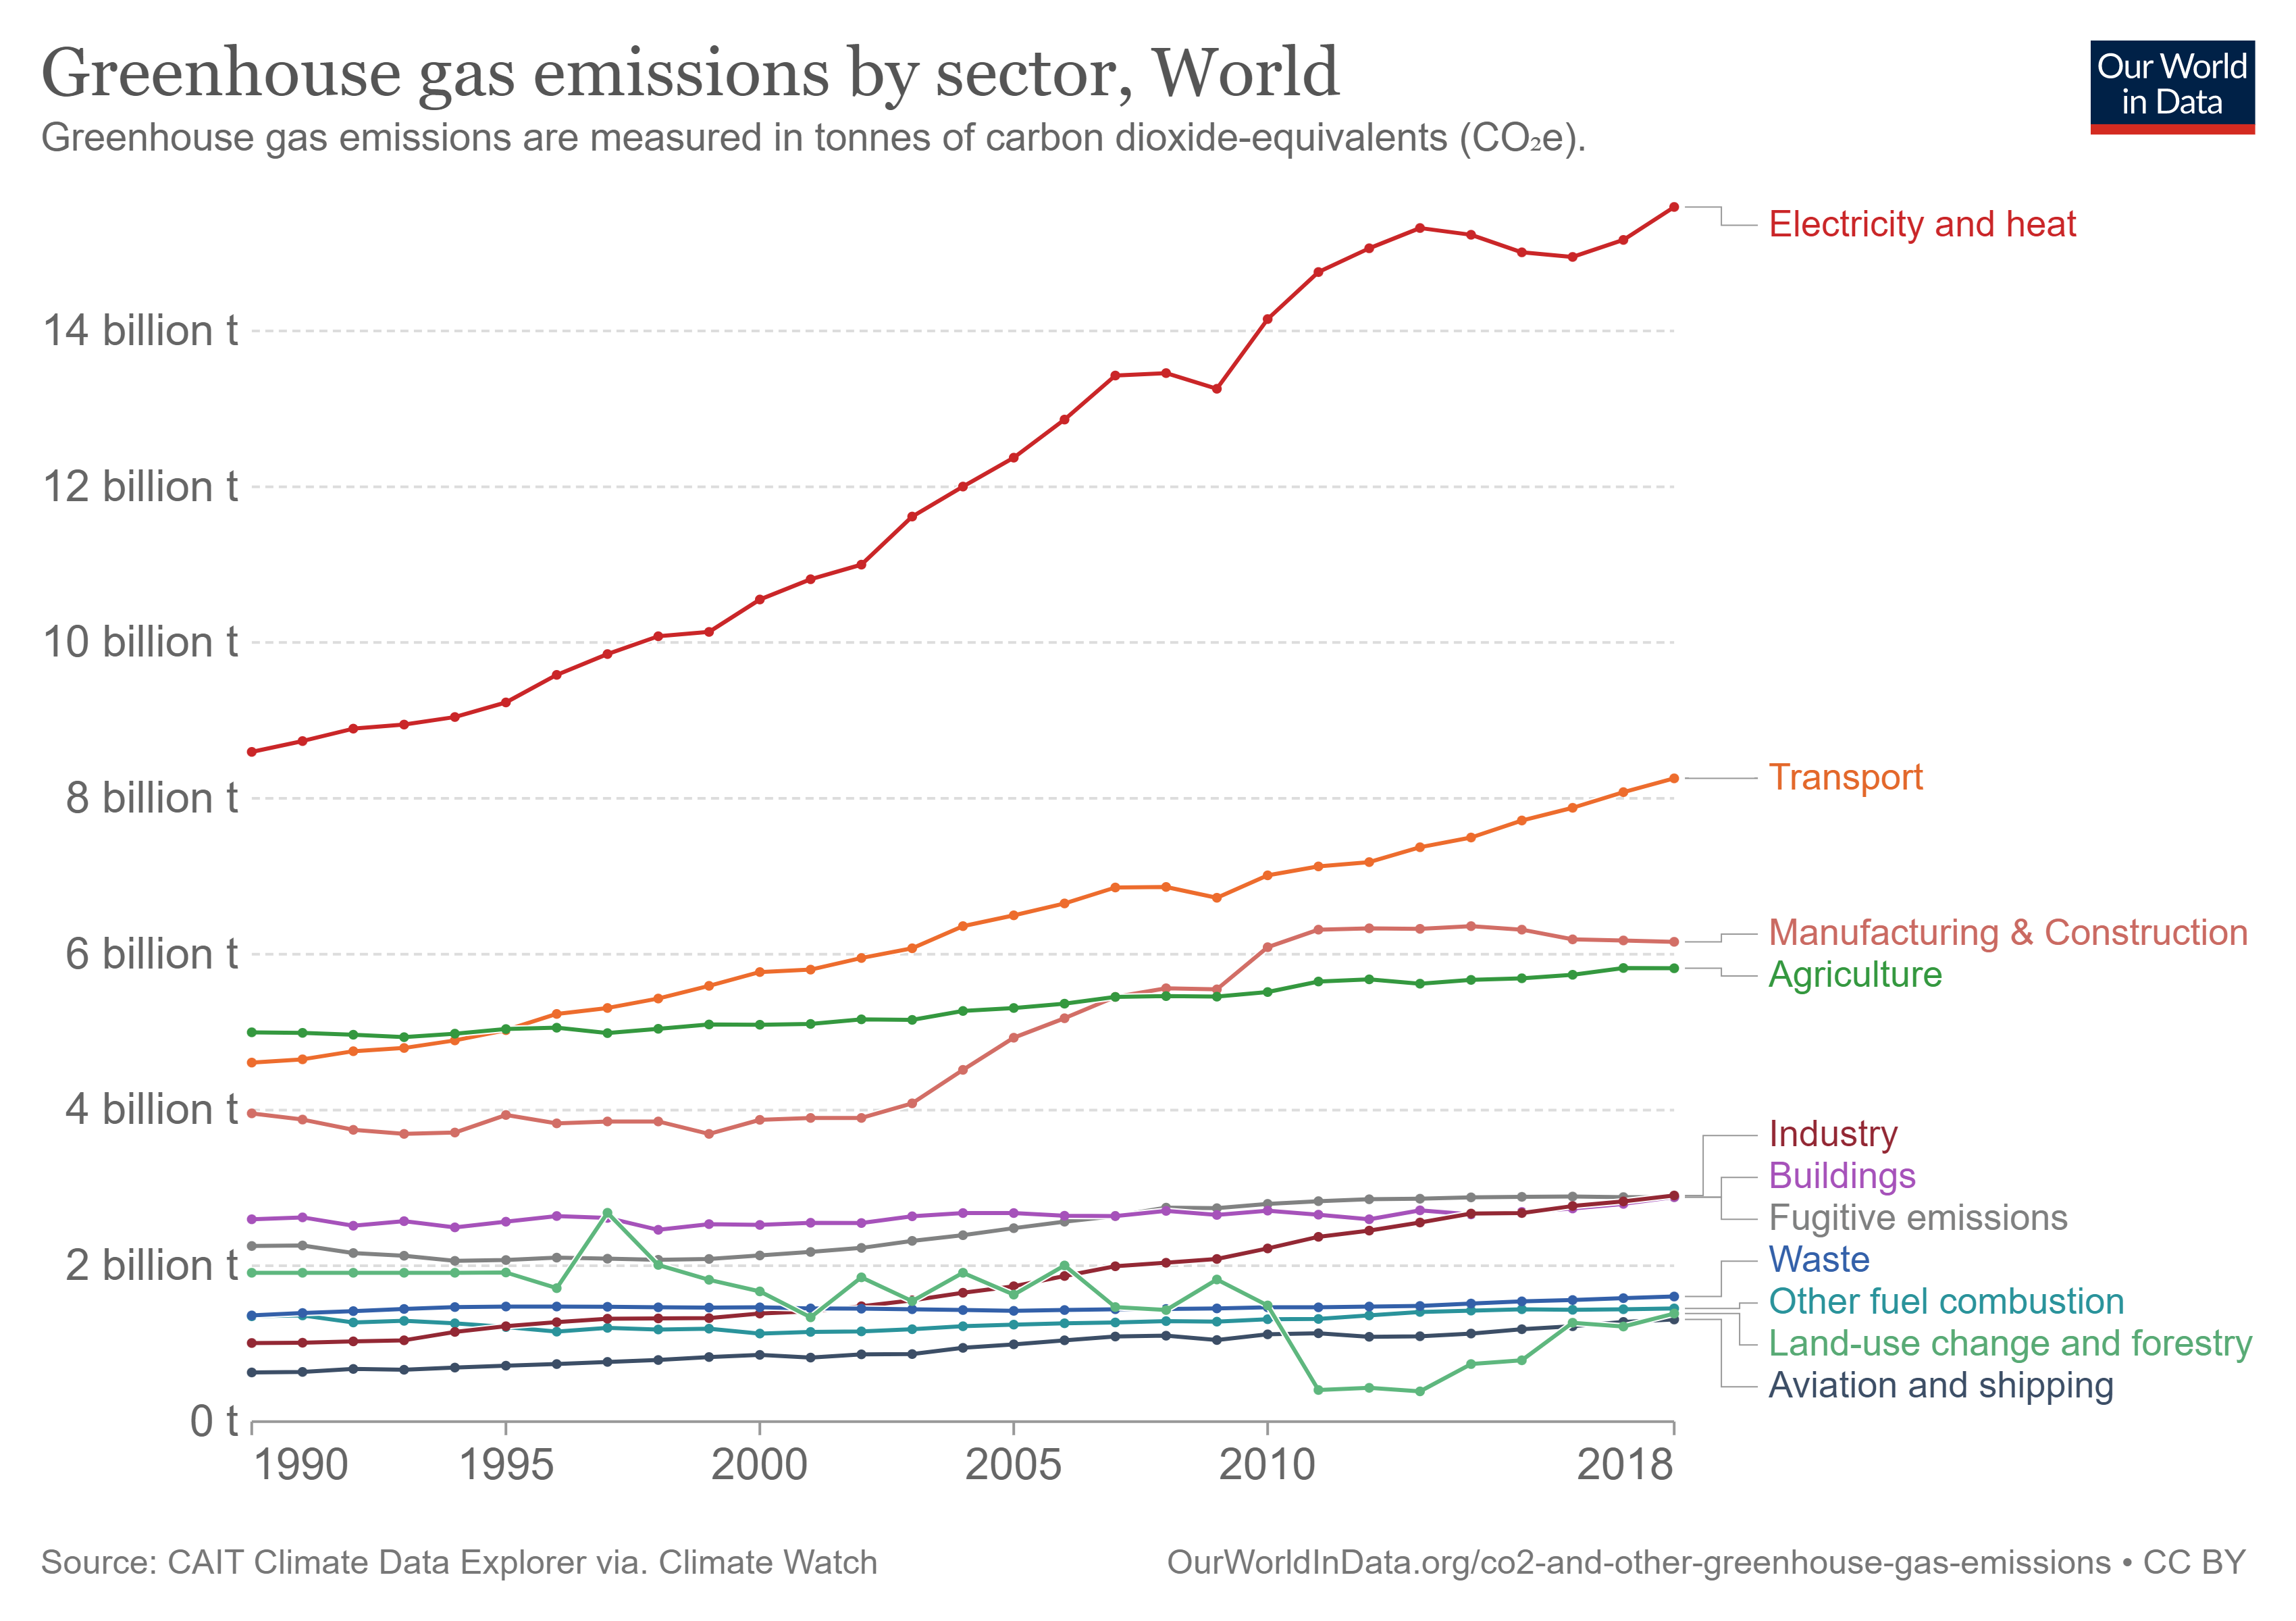
\includegraphics[width=\textwidth]{src/media/ghg-emissions-by-sector.png}
\caption{ghg Emissions by section}
\end{figure}

An estimated 5 trillion dollar for aquaculture alone \cite{goldman_sachs_hydrogen_2022} to reach net zero by 2050, this would imply that we require hydrogen for shipping, transportation, etc.


The potential of green hydrogen for is immense \cite{shipping_green_hydrogen}, for shipping it is an essential server. Companies like \index{ZIM} have already committed to using greener LNG, hydrogen is an natural extension of this.

From the water way technologies (\index{WATR.V}

Independent testing of the ESD system has demonstrated its capabilities. The tests targeted 85\% removal of specific compounds added separately to tap water. The target was achieved in all cases. \cite{cwti_esd}

Why Electro-static Deionization? 
\begin{itemize}
    \item Reduce TDS
    \item High removal efficiencies
    \item High water recovery
    \item No chemical additives
    \item Low maintenance
    \item Low energy consumption
\end{itemize}

\section{Fertilizer and CleanTech}

If the technology is as good as advertised, perhaps it just was not applicable until now, but given the latest new releases and their ability to generate green hydrogen. I believe its worth holding until 0.90 cents and forever in the tsfa accounts. Expected to hit a high amount under tax exemption, I believe with the canada water agency in 2022 good things are ahead for water investments.

Also trudeau pumping 12 billion into the "cleantech" space, there are not that many cleantech companies out there, but who wants to partner with the government, they have too much say in how things are run, and have their own agency that can change every 5 years.


 \begin{displayquote}
Customers prefer our regenerative products because they are made from natural mineral sources which are essential to the plant but do not leach into groundwater like conventional products. KSPC’s potash is an integral part of our blends and this LOI further establishes our long-term relationship and commitment to building the best soil health products possible - commented EarthRenew’s CEO, Keith Driver.
    \end{displayquote}
    
    
More research from the government of Canada's \cite{climate_change_2030_emissions} indicates support for fertilizer management which includes using organic and mineral fertilizer, EarthRenew fertilizer counts as organic which should be a huge plus. Also with the \$170 per ton carbon tax, Earthrenew should be able to grow faster by leveraging waste product, they should have a more friendly process.


\begin{blockquote}
Moving towards a circular economy can also increase the value of waste emissions through transforming raw material into fertilizers and renewable energy \cite{climate_change_2030_emissions}. EarthRenew plan to take waste and convert it to tangible fertilizer is incredible, aiming to hold for 5 years.
\end{blockquote}

The climate report from government of canada suggests that hydrogen production plants are similar in nature to oil refineries \cite{climate_change_2030_emissions}. Earthrenew having plants in Alberta is excellent.


\begin{figure}[h]
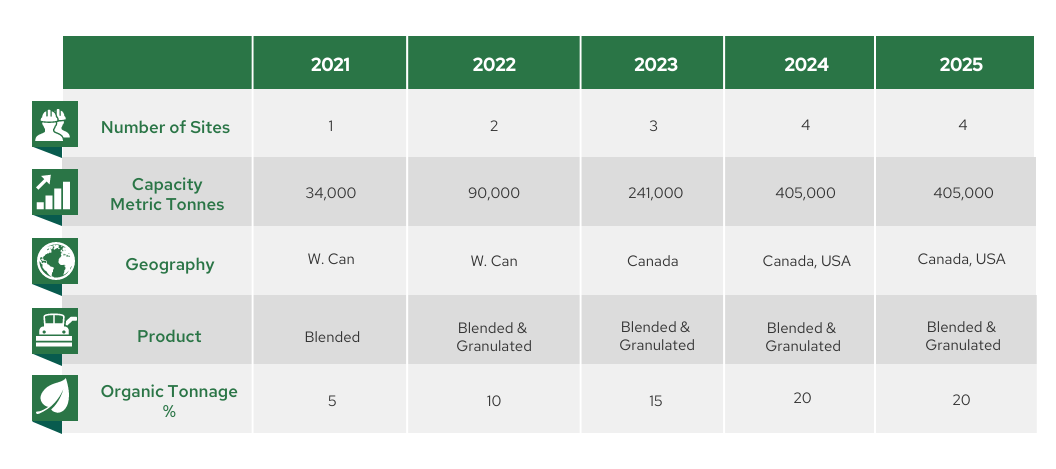
\includegraphics[width=\textwidth]{src/media/63894524-04fe-485b-a801-736431092c3c-e1633360733920.png}
\caption{Growth plan for earth renew}
\end{figure}

Selling their fertilizer along with the planned reduction of 30\% of emissions of fertilizer production in canada \cite{climate_change_2030_emissions}, it is very likely earth renew will get a lot of government support and do quite well. Based on their new releases they seem to be on track if not slightly behind.


\begin{blockquote}
The Government of Canada will continue to drive climate innovation by providing additional funding to
trial pre-commercial clean technologies and de-risk large-scale pilot projects critical to net-zero
transitions. Actions will be taken to enhance the Canadian climate innovation ecosystem to promote the
scale-up of clean tech companies and to coordinate efforts in strategic areas where it can yield major
emissions reduction \cite{climate_change_2030_emissions}. 
\end{blockquote}

Essentially the government is subsiding unproven companies like cielo, and/or helping fund earth renew, incredibly likely that earthrenew would qualify for free money.